\section{Development evidence for the hierarchical extension}
\label{app:shared}
An earlier internal study explored the hierarchical IRT line. Its generated tables, figure, and analysis script are included in the companion release~\citep{release}. We preserve those results here to explain why sharing evidence is a promising extension. These results use their own population, training split, and acquisition policies. Their ALC values describe that study; the selected submission's formative result remains 0.160822.

\paragraph{Study design.}
The development notes describe 52 development benchmarks in five domain-grouped folds and 20 hold-out benchmarks, with 20\% of evaluated model identities removed from training. The hold-out contains 654 subject--benchmark pairs and three seeds, giving 1,962 pair-seeds. It uses up to 400 evaluation items per pair; development runs use up to 100. The hold-out models are fitted on 160 training benchmarks. By comparison, the inspected \code{submit\_gate.zip} build records 180 benchmarks in its build inventory. The shared method connects these records, while their fitted states and evaluation populations remain distinct.

\begin{table}[H]
\centering
\caption{Preserved hierarchical development results from the committed main-result table. Dev and hold-out use different item caps. ALC columns reproduce the stored aggregate metrics. The last column first averages paired differences within each benchmark, then reports the mean and 95\% normal interval across 20 benchmarks. Consequently, it can differ from subtraction of the displayed ALC means. Bold identifies the selected hierarchical configuration in that study.}
\label{tab:shared-results}
\small
\setlength{\tabcolsep}{3pt}
\begin{tabular}{@{}lrrrrc@{}}
\toprule
 & \multicolumn{2}{c}{Brier ALC} & \multicolumn{2}{c}{Hold-out Brier} & \\
\cmidrule(lr){2-3}\cmidrule(lr){4-5}
Model & Dev & Hold-out & 0 labels & 31 labels & $\Delta$ vs. IRT \\
\midrule
Constant 0.5 & 0.2500 & 0.2500 & 0.250 & 0.250 & +0.0297\,{\scriptsize$\pm$0.0171} \\
Official baseline & 0.2523 & 0.2622 & 0.250 & 0.204 & +0.0380\,{\scriptsize$\pm$0.0110} \\
Lexical $k$NN & 0.2209 & 0.2291 & 0.250 & 0.201 & +0.0061\,{\scriptsize$\pm$0.0082} \\
CaimiraLite (static) & 0.2447 & 0.2603 & 0.260 & 0.260 & +0.0374\,{\scriptsize$\pm$0.0157} \\ \midrule
IRT (global evidence) & 0.2069 & 0.2202 & 0.260 & 0.194 & 0 \\
+ online item map & 0.1991 & 0.2154 & 0.260 & 0.185 & $-$0.0053\,{\scriptsize$\pm$0.0029} \\
+ subject regression, VI & 0.1979 & 0.2133 & 0.259 & 0.182 & $-$0.0076\,{\scriptsize$\pm$0.0046} \\
+ gate & 0.1959 & 0.2099 & 0.259 & 0.187 & $-$0.0108\,{\scriptsize$\pm$0.0046} \\
\textbf{+ acquisition radius 0.30} & 0.1939 & \textbf{0.2077} & 0.259 & 0.178 & $-$0.0132\,{\scriptsize$\pm$0.0044} \\
+ LLM difficulty prior & -- & 0.2066 & 0.258 & 0.178 & $-$0.0140\,{\scriptsize$\pm$0.0040} \\
\bottomrule
\end{tabular}

\end{table}

\paragraph{What the comparison contributes.}
The table records a progression from base IRT at 0.2202 ALC to the hierarchical gate with radius-0.30 acquisition at 0.2077. The development notes report gains on all 20 hold-out benchmarks and 75\% of pair-seeds. The largest added layer is the online item map: the benchmark-averaged ALC change is $-0.0053\pm0.0029$. This directly motivates learning relationships among items from the labels available on each new benchmark.

\begin{table}[H]
\centering
\caption{Preserved marginal layer effects from the committed ablation table. Each layer is compared with the preceding hierarchical stack. Differences and intervals use benchmark averaging. Win is the share of hold-out pair-seeds with lower ALC.}
\label{tab:shared-ablation}
\small
\setlength{\tabcolsep}{5pt}
\begin{tabular}{@{}lccc@{}}
\toprule
Layer added & Dev $\Delta$ ALC & Hold-out $\Delta$ ALC & Win (\%) \\
\midrule
+ online item map & $-$0.0059\,{\scriptsize$\pm$0.0030} & $-$0.0053\,{\scriptsize$\pm$0.0029} & 63 \\
+ subject regression, VI & $-$0.0007\,{\scriptsize$\pm$0.0015} & $-$0.0023\,{\scriptsize$\pm$0.0026} & 53 \\
+ gate & $-$0.0024\,{\scriptsize$\pm$0.0011} & $-$0.0032\,{\scriptsize$\pm$0.0026} & 68 \\
+ acquisition radius 0.30 & $-$0.0012\,{\scriptsize$\pm$0.0017} & $-$0.0024\,{\scriptsize$\pm$0.0023} & 57 \\
+ LLM difficulty prior & -- & $-$0.0008\,{\scriptsize$\pm$0.0011} & 62 \\
\bottomrule
\end{tabular}

\end{table}

The subject-regression/VI and signed-gate layers supply further reductions. The gate's reported late-budget tradeoff is visible in the original table: budget-31 Brier increases by 0.005 before widening the acquisition radius reduces it by 0.009. Prediction and acquisition therefore merit separate comparisons when joining this line with Rasch--CAIMIRA. The optional LLM-prior row is a separate research variant and adds external difficulty signals; the selected s44 archive and inspected gate operate locally.

\clearpage
\section{Interpreting the earlier development study}
\label{app:shared-scope}
\begin{figure}[H]
\centering
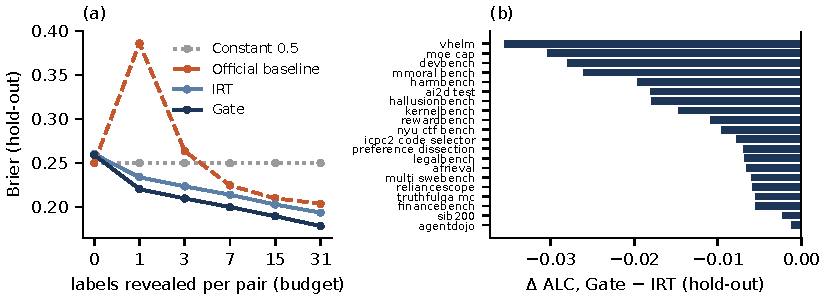
\includegraphics[width=\linewidth]{generated/fig_results.pdf}
\caption{Original generated figure from the shared development study, preserved byte for byte. Left: learning curves on its 20-benchmark hold-out. Right: per-benchmark Gate-minus-IRT ALC differences. The figure describes the hierarchical study in Appendix~\ref{app:shared}, separately from the nine-pair Codabench run in the main text.}
\label{fig:shared-original}
\end{figure}

\paragraph{Why the two model families fit together.}
Rasch--CAIMIRA provides a compact route from a subject's own labels to item-sensitive ability updates. The hierarchical model makes labels useful across related items and subjects within a benchmark. Its development results favor this shared evidence as labels accumulate. The proposed composition in Equation~\ref{eq:extension} asks whether both routes can support the same forecast: a strong initial prediction, a small pair-specific correction, and progressively richer shared structure.

\paragraph{The earlier external comparison.}
Earlier internal development notes also describe a Rasch-plus-rank-2 archive with 384-dimensional lexical features, evaluated on 19 hold-out benchmarks and 1,905 pair-seeds. Those notes report ALC 0.2217 for that archive and 0.2068 for the hierarchical gate, with a benchmark-averaged Gate-minus-external difference of $-0.0139\pm0.0072$. The external model has lower initial Brier score (0.248 versus 0.259), while the gate has lower endpoint Brier score (0.177 versus 0.202). The external model leads on five benchmarks: reliancescope, harmbench, rewardbench, moe\_cap, and preference\_dissection. That comparison also uses different acquisition policies: random for the external model and radius-0.30 for Gate. The observed strengths motivate a combined forecast under matched acquisition.

The earlier comparison omits devbench because byte-identical subject descriptors caused the external model to pool more than 31 labels and raise an error. The selected s44 source likewise matches support by the full subject dictionary and enforces a 31-label limit. An exact archive hash and the pair-level replay records would establish whether the earlier external result belongs to this selected ZIP. That identity remains \textbf{UNVERIFIED}; the figure and tables above characterize the hierarchical study, while the exact-hash component comparison in Table~\ref{tab:local} supplies the selected candidate's local evidence.

\paragraph{Reproduction path and study scope.}
The original \code{make\_numbers.py} reads \code{pairs.csv} and \code{metrics.json} for each run under \code{../runs/}. It computes matched contrasts using subject, benchmark, and seed as keys, averages differences within benchmarks, and forms normal intervals across benchmarks. Its tables, figure, configuration summary, and generation code are included under \code{paper/} in the companion repository. The new compact appendix tables select columns from those same committed rows.

The companion package contains those generated outputs and the script; the underlying raw run files remain outside the package. Full result regeneration and archive identity matching remain separate evidence steps. The development notes record four looks at the hold-out during stack selection and gate weights fitted on an earlier development split. These details bound interpretation while preserving the study's central contribution: shared item structure offers a measurable and interpretable direction for extending sparse adaptation.
